% Chapter 4

\begin{savequote}[45mm]
$pV \neq nRT$ 
\qauthor{The universal gas law does not apply to supercritical fluids}
\end{savequote}

\chapter{Instrumentation: Supercritical Fluid Chromtography} % Main chapter title

\label{Chapter4} % For referencing this chapter elsewhere, use \ref{Chapter4}

This thesis discusses the development of a comprehensively coupled
(supercritical fluid × gas) chromatograph and its application to the analysis of
biodiesel. The discussion on the experimental work divides naturally into two
parts: this chapter discusses the supercritical fluid chromatography (SFC) and
the next chapter discusses the gas chromatography (GC).

\section{SFC}

As discussed in Chapter \ref{Chapter2}, an SFC chromatograph consists of a
supply of mobile phase, a pump, a pressure control system, a modifier control
system, a column, a pressure relief system and a detector

\subsection{Mobile phase}

As mobile phase we used carbon dioxide. The benefits of carbon dioxide as an
solvent and mobile phase is discussed in Chapter \ref{Chapter2}.

We used 99.995 \% pure carbon dioxide supplied by Air Produts. Our colleauges in
industry also uses food grade or technical grade carbon dioxide and they have
not reported any significant impurities.

As modifier we used LiChrosolv\textregistered methanol from Merck. This is an
`HPLC-grade' solvent, of which the purification is optimized for the removal of
UV-absorbing impurities. Using this grade of solvents is important when using
optical aborbance or fluorescence detectors, because low levels of impurities
improve limits of detection.

It is quite likely that less a expensive grade of modifier would be suitable for
our SFC, because we do not use an optical detector. HPLC-grade solvents does not
have an effect on the quality of the chromatography.

\subsection{Pump}

As pump we used a Varian 8500 HPLC pump. This pump had its control electronics
removed, and it was controlled from a personal computer by software written for
the purpose.

The Varian 8500 pump was driven by a stepper motor. This kind of motor turns in
discrete steps, instead of at a constant rate. It is driven by pulses of
electric current, rather than a continuous current, and therefore the speed of
the motor can be controlled by varying the rate of the pulses. This makes it
relatively simple to control the speed of the motor from a computer.

The Varian 8500 pump has a built-in pressure transducer that provided an
electronic signal proportional to the pressure at the pump outlet.

The Varian 8500 pump is a piston pump with a 250 \si{\milli\litre} capacity that
needs to be refilled between strokes. Refilling means that one has to stop
chromatography, which makes it important to fill the pump to full capacity, so
that chromatographic runs are not interrupted. This means that the pump needs to
be filled with carbon dioxide in the liquid phase rather than the vapour phase.
Compressing either would create the appropriate phase for doing chromatography,
but compressing a vapour phase would leave one with a much smaller volume of
high-pressure carbon dioxide than compressing a liquid phase.

Filling a pump with liquid carbon dioxide might be more difficult than one would
imagine. 


\begin{figure}
\centering
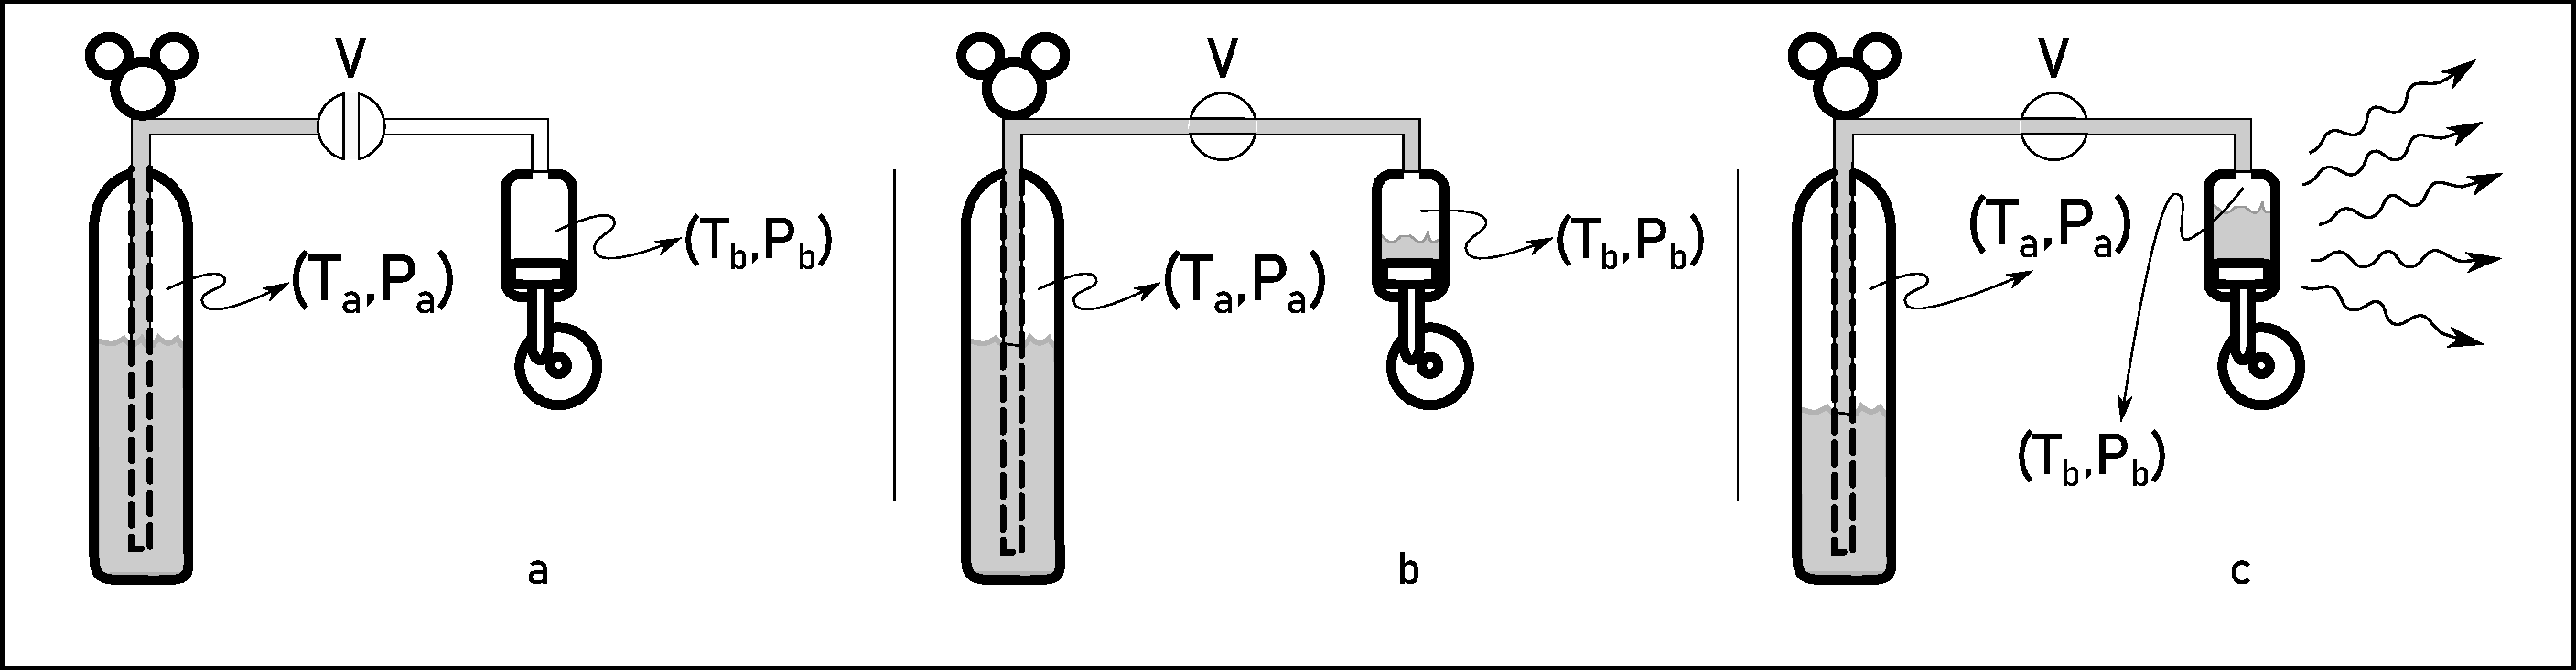
\includegraphics[width=\textwidth]{Figures/CO2Filling.pdf}
\decoRule

\caption[Fillng a CO\textsubscript{2}]{Diagram to help explain the filling of
the carbon dioxide pump. (a) Reservoir with high-pressure liquid carbon dioxide
(b) Receptacle for carbon dioxide (V) Valve.}

\label{fig:co2fill}
\end{figure}

Imagine a reservoir of liquid carbon dioxide (a), equipped with a dip tube,
connected to an empty receptacle (b) via a valve (V). (See Figure
\ref{fig:co2fill}) One can assume that the receptacle is empty and contains only
carbon dioxide vapour at atmospheric pressure, say 1 atm. The vapour pressure of
the vapour about the liquid in the reservoir (a) is about 55.3 atm (5.6 MPa).
When the valve (V) is opened the will high-pressure vapour in the reservoir (a)
will expel the liquid carbon dioxide through the dip tube and through the valve,
into the receptacle (b). This process will continue until the vapour pressure in
the receptacle is the same as the vapour pressure in the reservoir.
A certain amount of boiling will occur, until the pressure has equalized. The
system will now be in equilibrium, and there will be no flow of liquid carbon
dioxide. One can attempt to now increase the flow by increasing the volume of
the receptacle (for example by withdrawing a pump piston), and hence
decreasing the vapour pressure there. But any flow from the reservoir will lead
to expansion of the headspace of the reservoir. This will lead to cooling of the
headspace, and therefore lower pressure and therefore lower flow. The final
result of this process is that the receptacle is never filled to capacity with
liquid.

The way to fill the reservoir to capacity is to ensure that the temperature of
headspace vapour $$T_a$$ higher than the temperature of the headspace vapour
$$T_b$$. Because safety regulations prohibit the heating of a cylinder of
pressurized gas, the thing to do ensure $$T_a \lt T_b$$  to cool the receptacle.
This cools the headspace vapour, and following Gay-Lussac's law the pressure
$$P_a$$ decreases, the difference $$P_b - P_a$$ increases and the liquid flows
until the receptacle is filled to capacity.
 
In the case of the Varian 8500 pump the cooling of the pump was achieved by
wrapping a coil of copper tubing around the cylinder, and pumping a
heat-exchange fluid through it. A chiller with a mechanically cooled tank with a
20 l capacity was filled with a solution of 7.5 l of diethyl glycerol and 7.5 l
of water. This mixture has a freezing point of -10 \degreeCelsius, which can be
cooled by the chiller without freezing. (If the coolant freezes a layer of ice
forms on the cooling plate of the chiller, which isolates the remaining liquid
from the cooling plate and limits the temperature of the coolant to the melting
point of the coolant.) An inexpensive submersible water pump (designed for
decorative water fountains) was used to pump the coolant through the circuit.
This pump can deliver 800 l of water per hour at a head of 1.2 \si{\metre}.

For some experiments we also used a SFT-10 pump from Supercritical Fluid Technologies (Newark,
Delaware). This is a purpose-built two-piston pump with a sapphire pistons and a
Peltier-cooled head. This is a much better technology than the HPLC pumps. It
takes up less space and does not need refilling, since it feeds directly from
the cylinder. This pump had it's own microprocessor controllers on board,
and flow and pressure could simply be commanded from the PC through a USB cable. 



\subsection{Pressure control system}

In chromatography the figure of merit by which the performance of a system is
measured is the distance by two compounds are separated. This is known as the
\textit{resolution}. The efficiency of the system is often expressed as the
\textit{theoretical plate height}. But the days of separating coloured compounds
in glass packed columns are long past and the direct measurement of distances
are now relegated to thin-layer chromatography. Instead, we have to make do with
proxy values such as \textit{retention volumes} or \textit{retention times.}

Retention times are particularly convenient today, because it can easily be
measured by computer systems.

Retention times, however, depend on a known flow rate of the mobile phase
through the column. The flow rate need not be constant, although for the sake of
simplicity a constant flow rate is preferred. Ideally, the flow rate should also be
adjustable.

The need for an adjustable, constant flow rate can be met by using a control
system. Control systems are well understood by engineers, among whom it is a
major field of study \autocite{Koenig2009}. 

Figure \ref{fig:processcontrol} shows a diagram of a simple process control
system. Some aspect of the process under control is measured, which yields the
\textit{process variable} (PV). The PV is compared to the \textit{set value}
(SV), and the \textit{error} (e) obtained by finding the difference. The error
is provided to the controller, which calculates the \textit{manipulated
variable} (MV). The MV is used to drive the final control element, which adjusts
the process with the aim of producing a smaller error.

\begin{figure}
\centering
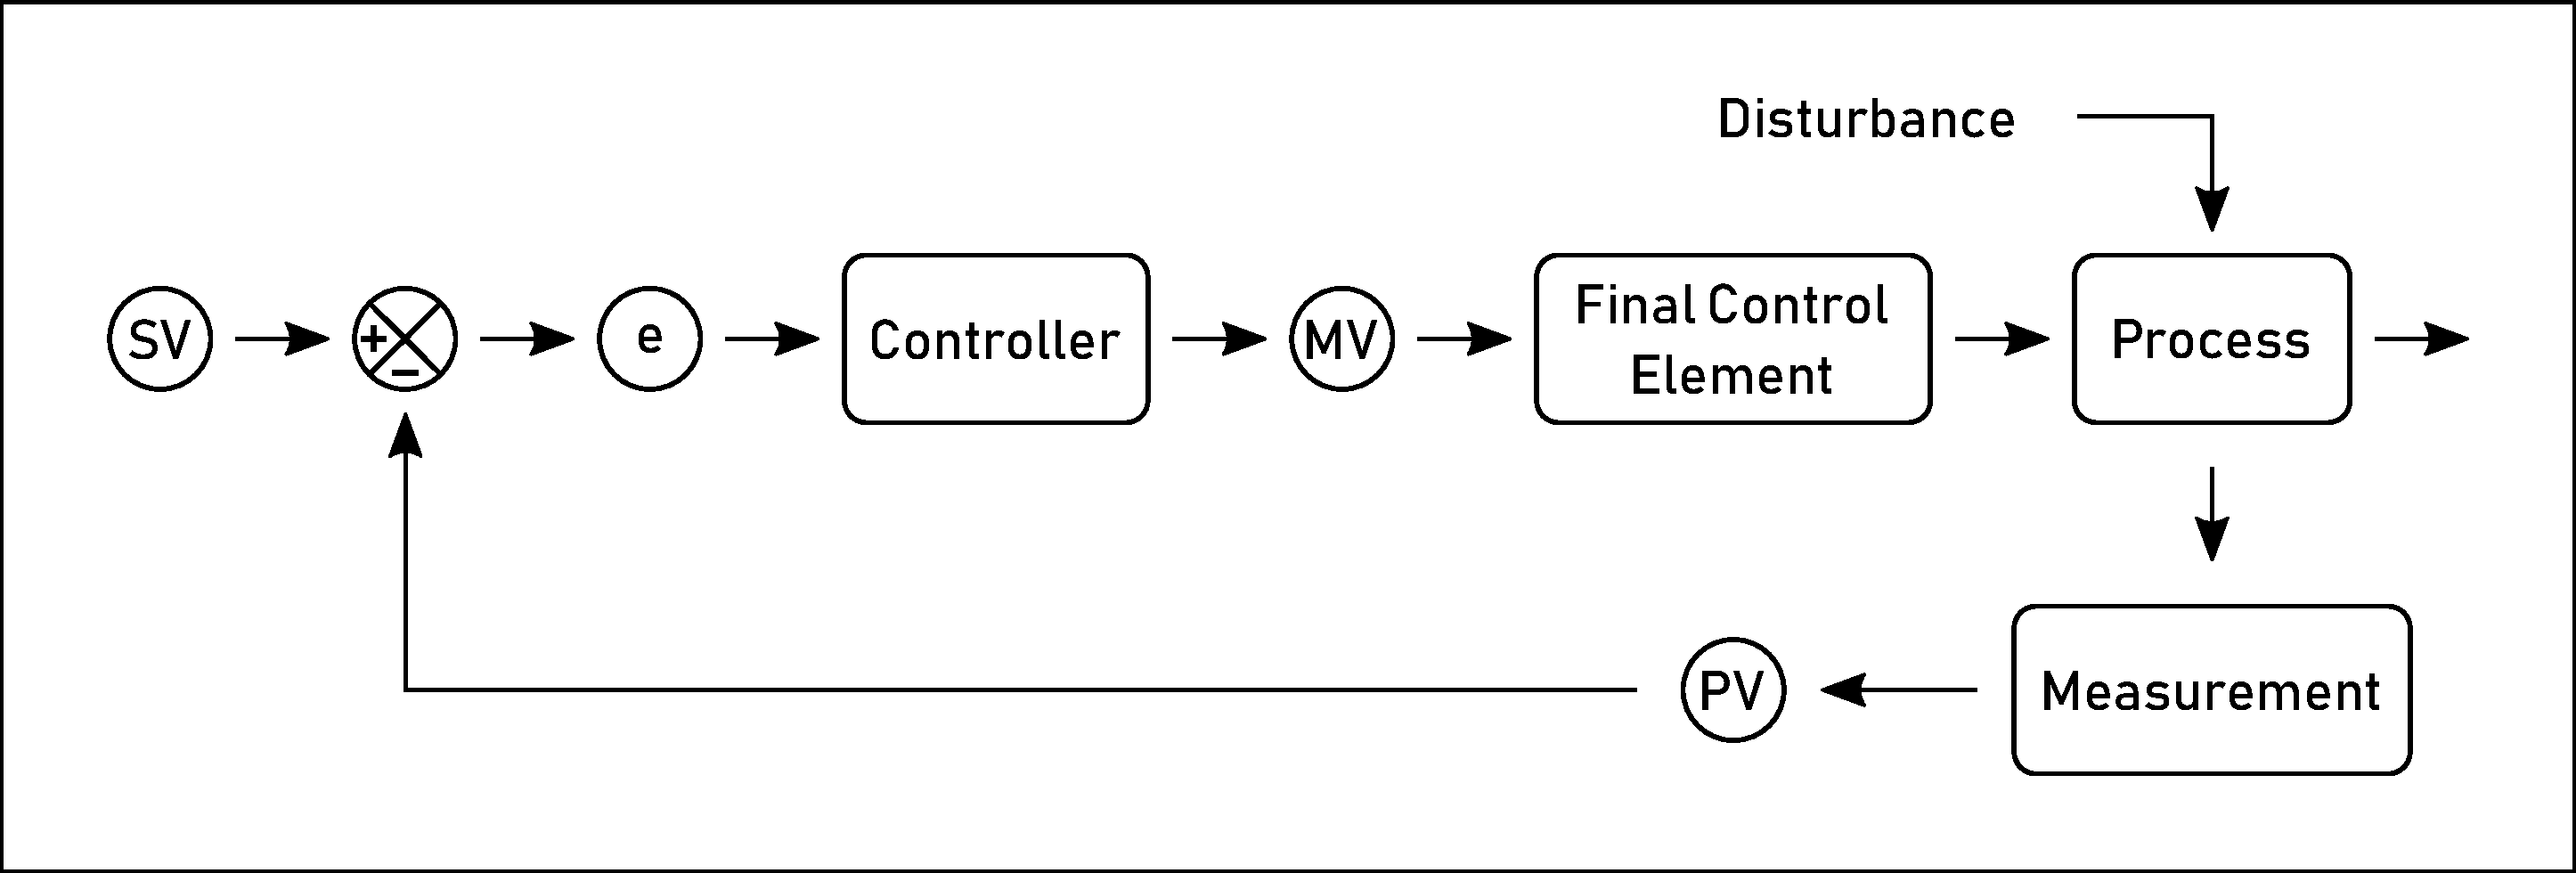
\includegraphics[width=\textwidth]{Figures/ProcessControl.pdf}
\decoRule

\caption[A process control system]{Schematic diagram of a closed-loop control
system. (SV) Set Value, (PV) Process Variable, (e) Error, (MV) Manipulated
Variable}

\label{fig:processcontrol}
\end{figure}

Chromatographic systems conventionally works under pressure control or flow
control regimes. Either is suitable: constant pressure systems usually yield
constant flow if other parameters are held constant. Because flow measurement is
more complex than pressure measurement, pressure control is the older, simpler
and less expensive control method. We therefore selected pressure control as our
control regime.

In our system the pressure measured by the on-pump sensor was the process
variable (PV) . This was compared to the set value (SV) set on the computer
console. The controller was a software algorithm, implemented as a virtual
instrument in the programming environment LabVIEW. The controller computed an
output value for the manipulated variable (MV), which was the rate at which
pulses were sent to the pump, in hertz. The digital input/output (DIO) interface (National Instruments PCI-136)
created those pulses and sent them to the pump's electronic interface.

The software used a PID (Proportional-Integral-Derivative) controller module,
with the Integral and Derivative contributions disabled. While enabling the
Integral and Derivative contributions would add to the accuracy of the
controller, we could not find a suitable, simple tuning procedure. Tuning the
controller from adequate performance to optimum performance would consume
resources while not improving chromatography.

\subsection{Modifier Control}

The modifier needs to be present in the mobile phase at a known and controlled
concentration.

There are various SFC-modifier mobile phase supply units on the market. They
tend to be a expensive and complex, because they require the use of two
controlled, high-pressure pumps. Given that our needs were rather modest, we
elected to use a simpler system.

Instead of accurately pumping two fluids, that means the supercritical fluid
and the modifier, we only pump and control the supercritical carbon dioxide and
add measured volumes of modifier.

The modifier control unit consisted of a six-port valve, a fixed-volume
measuring loop, and a mixing chamber. 

The unit operates by filling the measuring loop with modifier, and then
switching the measuring loop into the flowing mobile phase. This is followed by
a waiting period during which the mobile phase washes the modifier out of the
measuring loop. The modifier is washed into the mixing chamber, where it is
intimately mixed with and dissolved in the supercritical carbon dioxide. The
concentration of modifier in the mobile phase is determined by the switching
rate of the sampling valve. Given that about 3 volumes of supercritical carbon
dioxide is needed to wash the modifier out of the loop, the highest
concentration of modifier that can be added in this manner is about 25 \%.
Beyond this the approximations behind the calculations no longer hold.

Figure \ref{fig:mixingchamber} shows the chosen design of the mixing chamber.
The inlet and outlet pipes of the mixing chamber extend far into the chamber, to
encourage turbulent flow. 

\begin{figure}
\centering
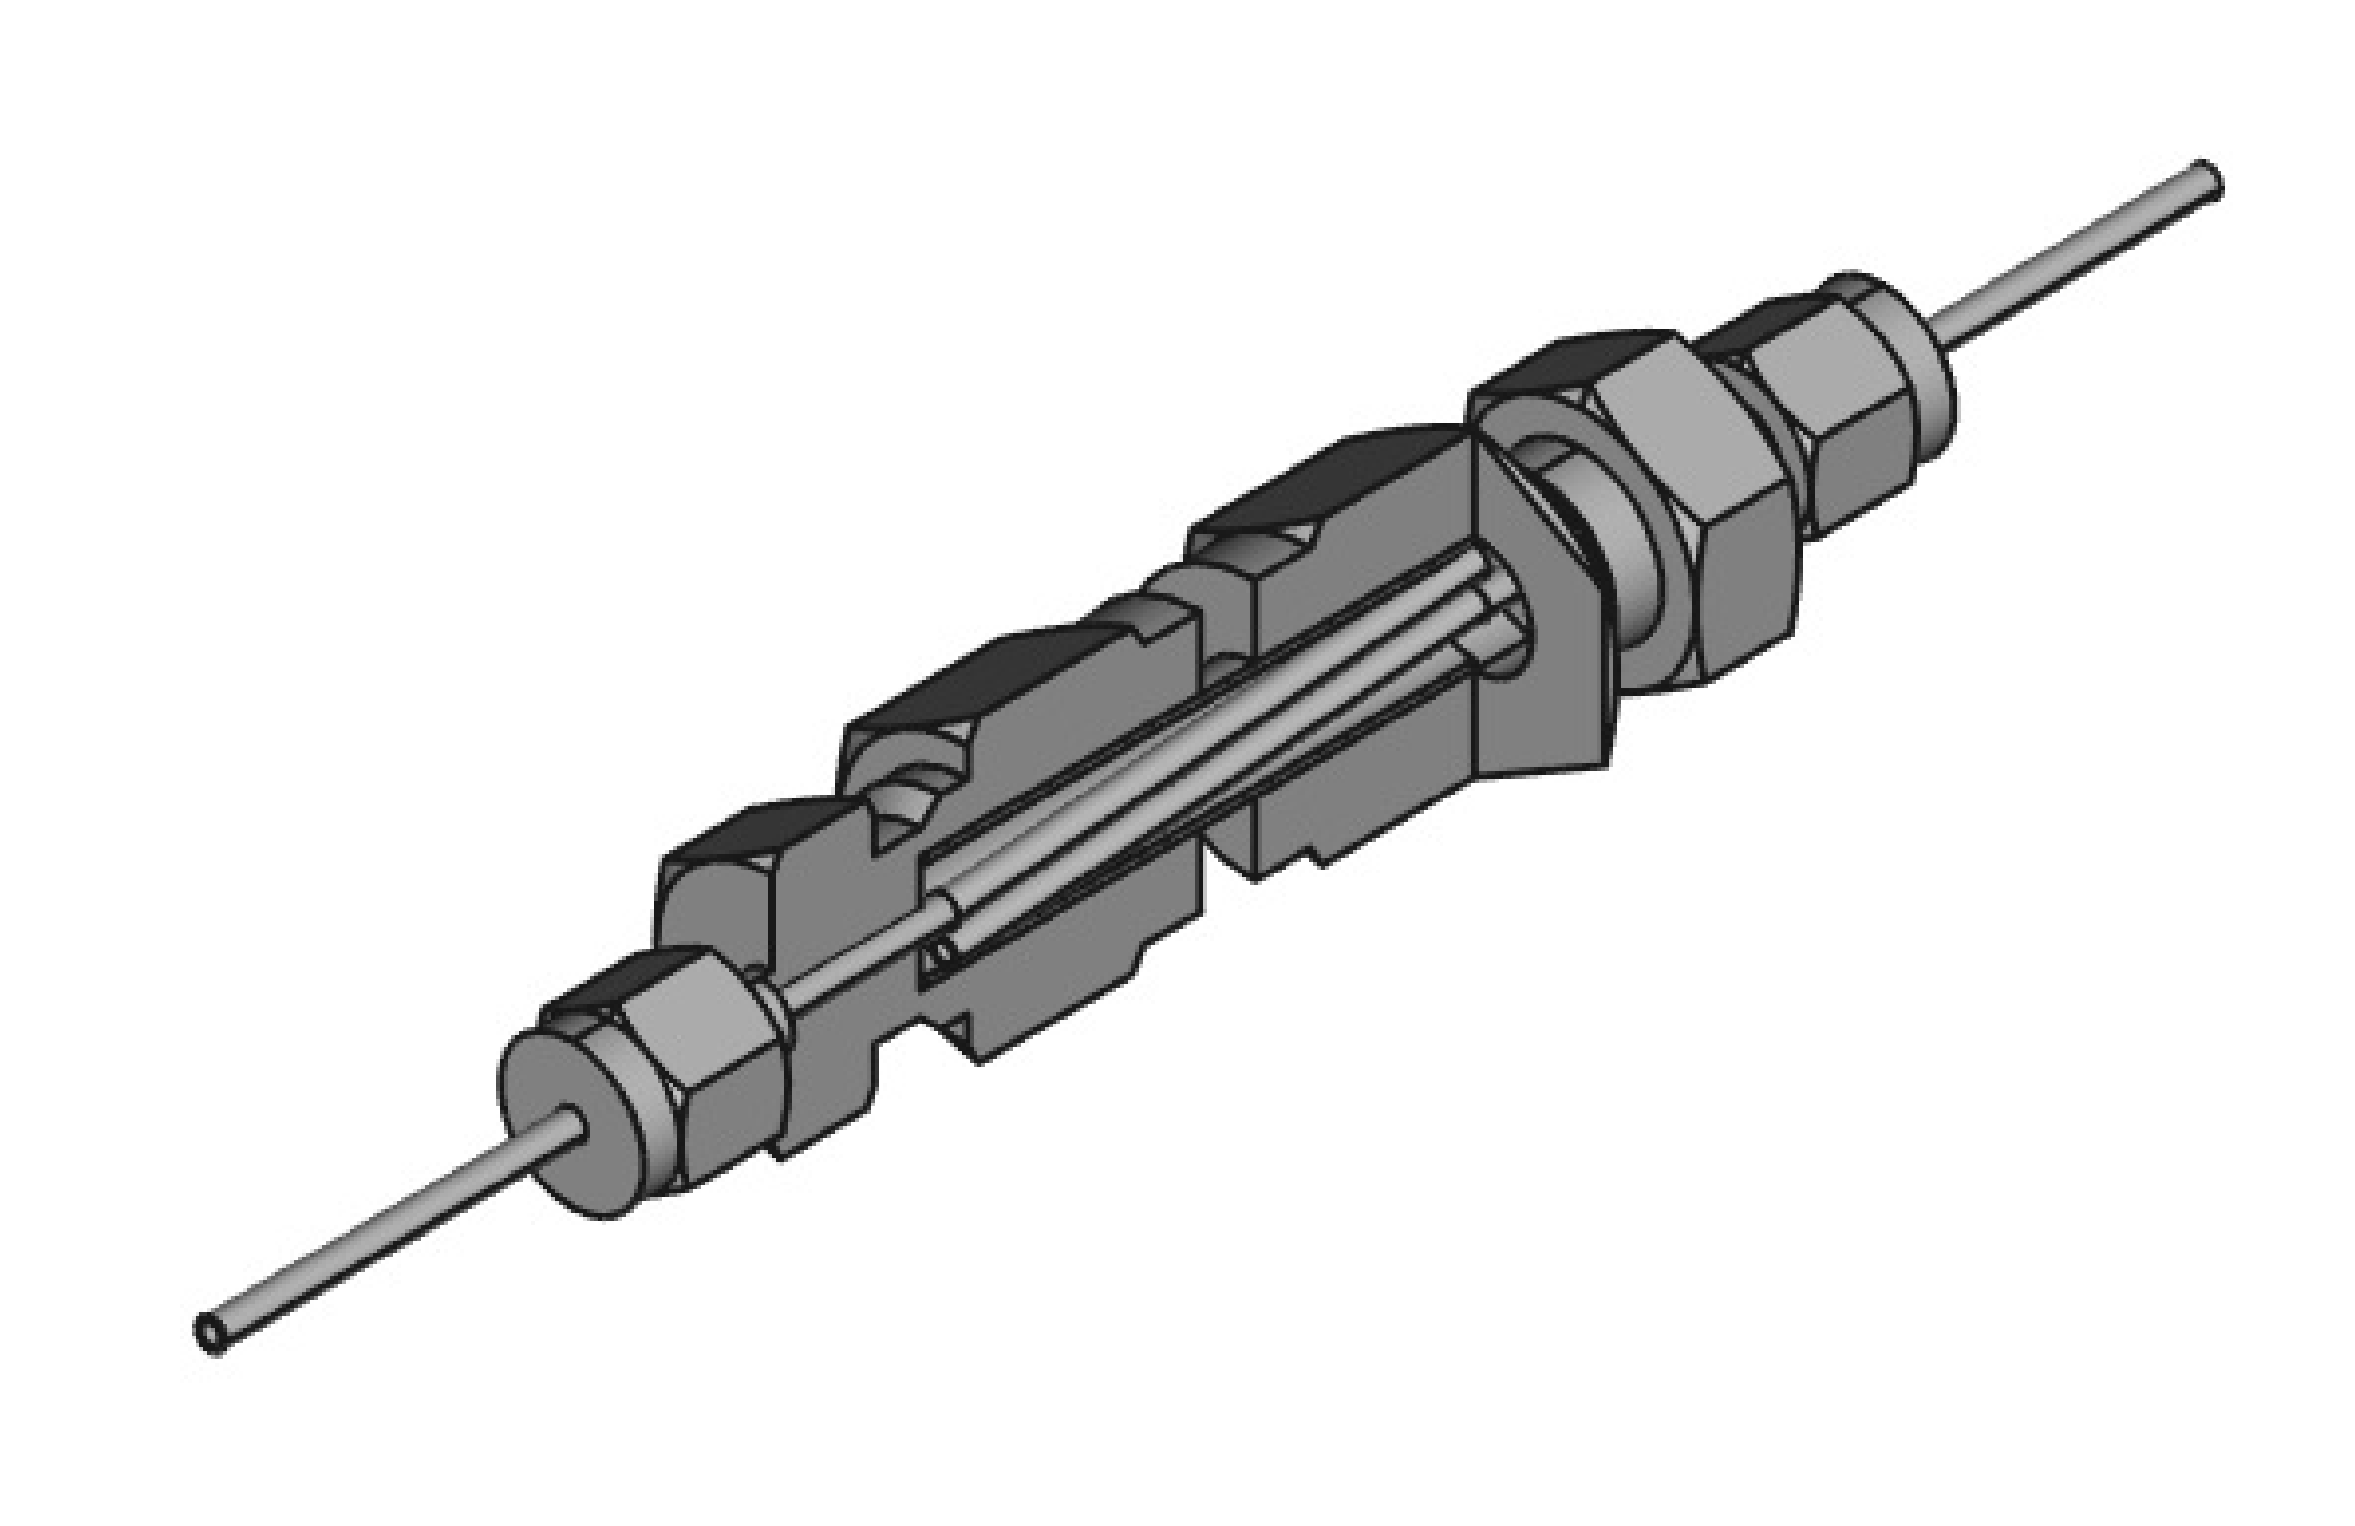
\includegraphics[width=\textwidth]{Figures/MixingChamber.png}
\decoRule

\caption[A cutaway diagram of the mixing chamber]{A cutaway diagram of the
mixing chamber design. The chamber is designed for the mixing of the modifier
and the supercritical carbon dioxide.}

\label{fig:mixingchamber}
\end{figure}

The modifier injection valve position was commanded from the controlling PC by electronic
voltage pulses.

\subsection{Sample injection}

The sample inlet was a two-position valve with an internal sampling volume
(Figure \ref{fig:samplingvalve}). In one position the sampling volume was filled
with a syringe, and when the valve was commanded to inject the sampling volume
was switched into the carrier mobile stream.

\begin{figure}
\centering
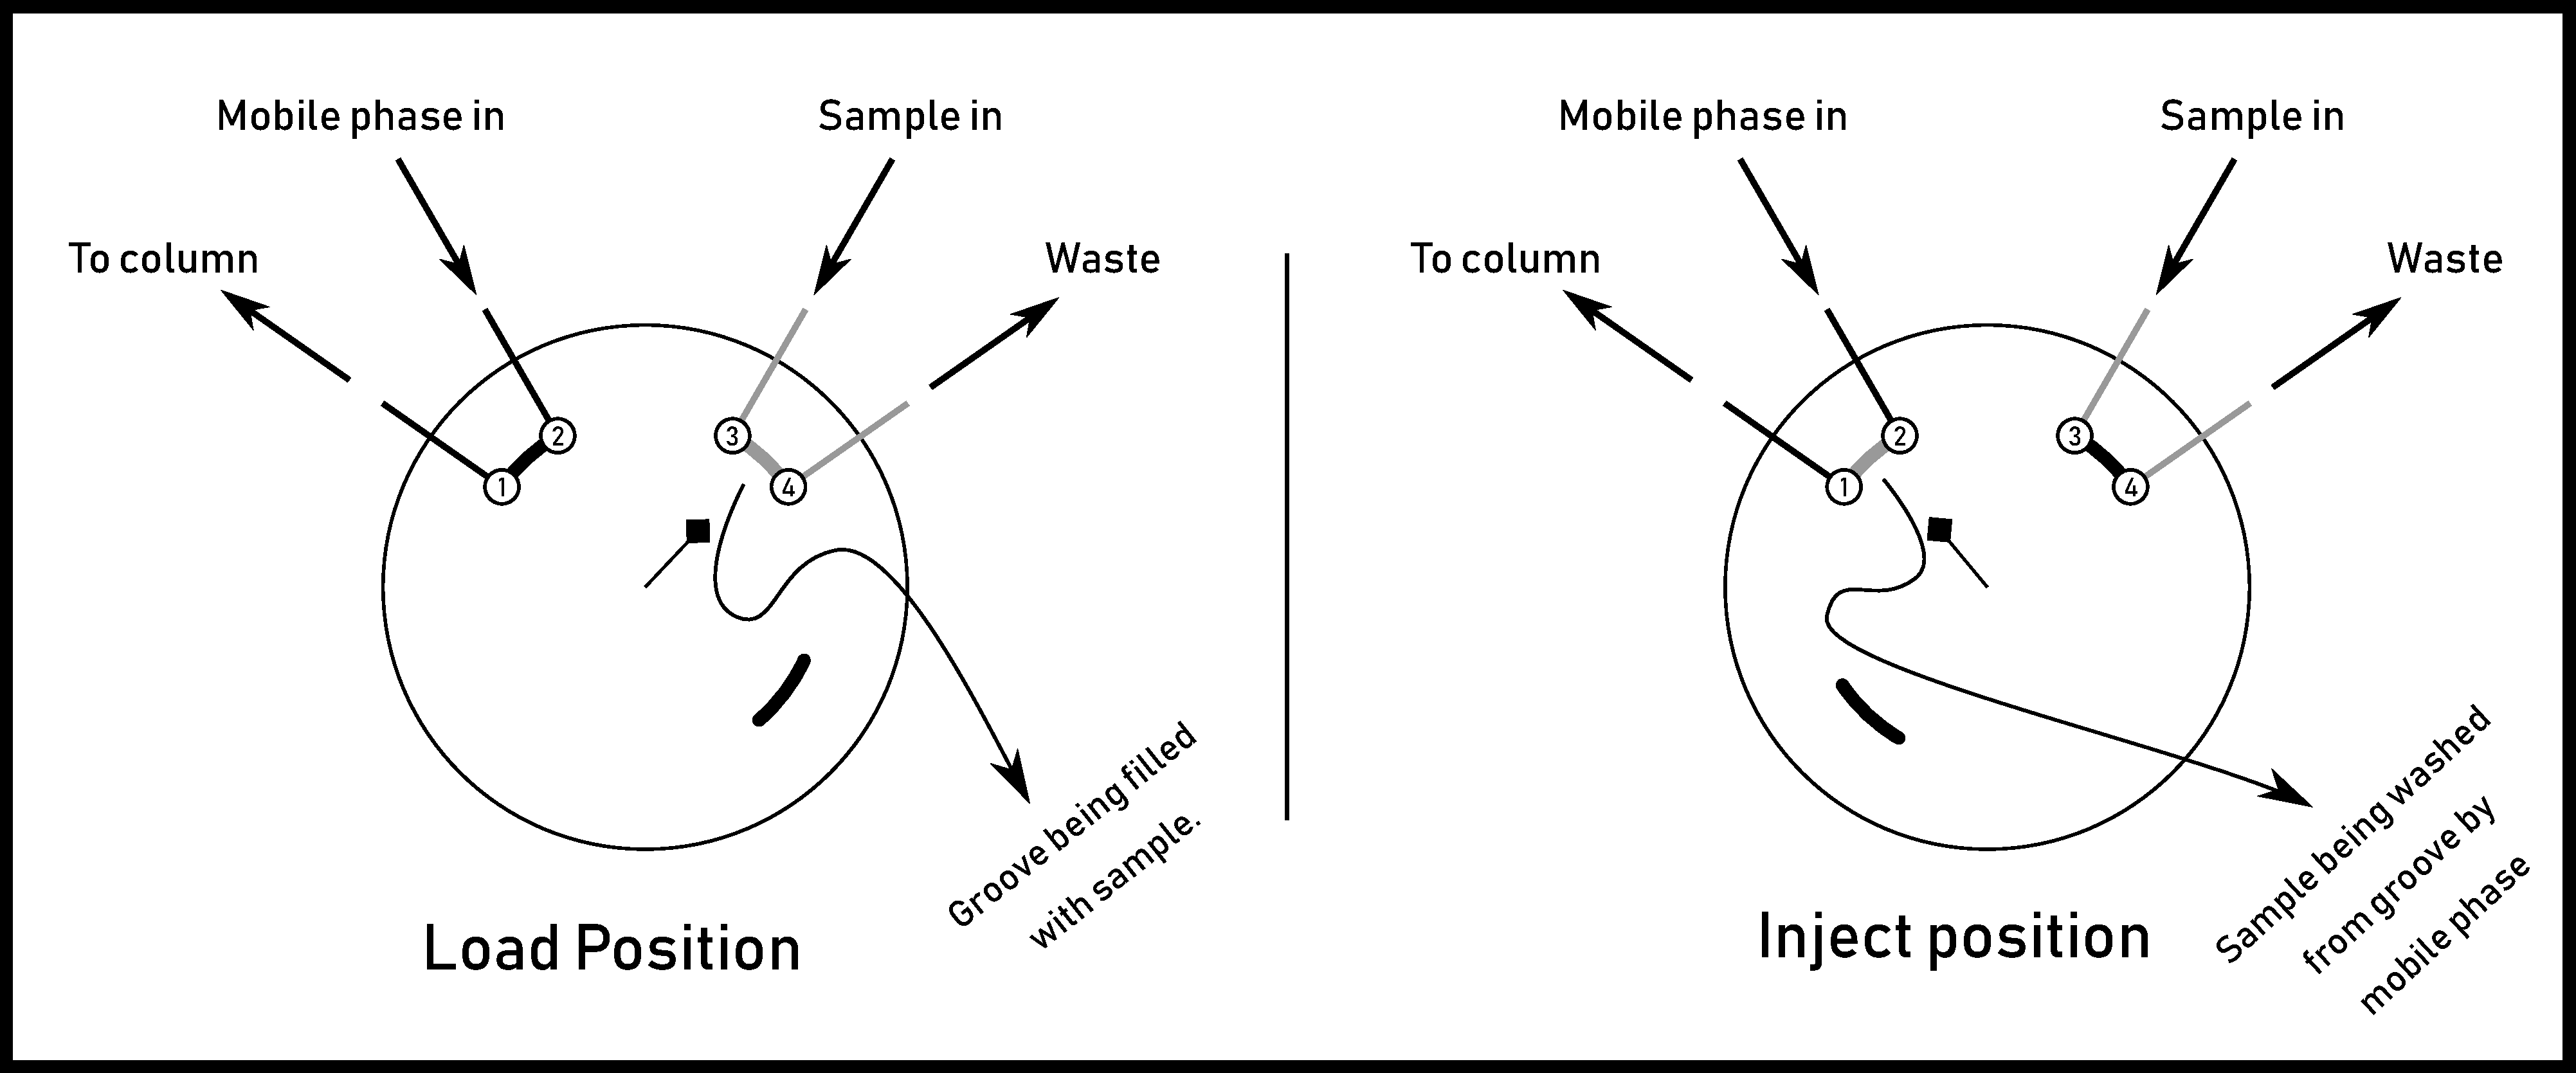
\includegraphics[width=\textwidth]{Figures/SampleValve.pdf}
\decoRule

\caption[Schematic diagram of the injection valve.]{A schematic diagram of the sampling valve. }

\label{fig:samplingvalve}
\end{figure}

The reader might be more familiar with the six-port valve as an injection
system. The benefit of the internal groove injection valve is that it allows a
much smaller volume to be injected. Using this small volume makes it possible to
inject samples without dilution, which simplifies sample preparation.

The sample volume was 5 $\mu$l

The injection valve position was commanded from the controlling PC by electronic
voltage pulses.

\subsection{Column}

The separation power of a chromatographic system can be modelled by the equation 

\begin{equation}
R_s = \bigg(\frac{\sqrt{N}}{4}\bigg)  \bigg(\frac{\alpha-1}{\alpha}\bigg)  \bigg(\frac{\bar{k}}{1+\bar{k}}\bigg)
\end{equation}

were, $$R_s$$ is the \textit{peak resolution}, $$N$$ is the \textit{number of plates}, $$\alpha$$ is the \textit{separation factor}, and $$\bar{k}$$ is the \textit{retention factor}.
 
The number of plates $$N$$ can be increased simply by making the column longer,
at the cost of increasing the time of the run.

The maximum length of the column is determined by the pressure drop available
that will still yield adequate flow. In capillary gas chromatography the
openness of the column and the low viscosity of the gas-phase mobile phase
routinely allows columns that are 100 metres long at inlet pressures of a few
atmospheres. In HPLC the high viscosity of the mobile phase and the narrow,
tortuous pathways between the small particles means that the columns are
typically 100 - 200 mm long, requiring hundreds of atmospheres of inlet pressure
for adequate flow.

The low viscosity of an SFC mobile phase makes it possible to used packed
columns, such as those developed for HPLC use, but make them much longer. This
allows us to have a higher number of plates in the chromatographic system at the
cost of nothing more than a longer column.

The SFC column we used in the SFC×GC system was a set of 5 HPLC columns (150 mm
$\times$ 4.6 mm, 3 $\mu$m particles) (Restek, Pinnacle DB Silica) connected in
series.

The stationary phase in this column is `bare silica', which is 'polar'. That
means that the packing of the column consists of particles of silica with no
organic phase covering its surface, and hence one that will interact strongly
with polar molecules. In contrast, a `C18' stationary phase is 'non-polar'. The
particles of such a stationary phase are coated with octadecyl chains bonded to
its surface, and hence will tend to interact strongly with non-polar molecules.
The base material of the particles is usually silica, but that is because
creating uniform particles of a given size from silica is a mature technology. 

\subsubsection{Stop-flow}

The convention for chromatography is to run

\subsection{Pressure Relief}

No matter the kind of SFC system one uses, at some point the elaute needs to be
depressurized. This can be before or after the detector. If depressurization
happens after the detector, then the details of the mechanism doesn't matter
much, because the information has been obtained and the eluate can be
discarded. If, as in our case, the depressurized eluate needs to still pass the
detector, it is important to not lose the resolution achieved by the column.
This means that the design of the depressurizer requires some care.

The main concern in depressurizer design is premature desolvation of analytes. This
causes \textit{discrimination}, which is the differential treatment of
substances where identical treatments are expected. In particular, molecules of
higher molecular weight is easier to desolve from the supercritical fluid, and
might precipitate if the depressurizer is not designed to prevent that.

Depressurization can be done either statically or dynamically. In a dynamic
system there is an active element that controls the flow of the eluate in such a
way as to maintain the pressure before the active element at a certain level.
Such a device is often called a \textit{back pressure regulator}, and is usually
an electro-mechanical device with digital control. They tend to be complex and expensive. 

In static depressurization there is no active pressure control. A simple
\textit{restrictor} is used to limit the flow between the high pressure of the
SFC and the low-pressure outlet. 

Textbooks often discuss different restrictor designs, for example
\autocite{LuquedeCastro1994}. Our preferred depressurizer was the `integral' or
Guthrie design \autocite{Guthrie1986}. Figure \ref{fig:restrictor} shows the steps
in manufacturing the Guthrie restrictor.

\begin{figure}
\centering
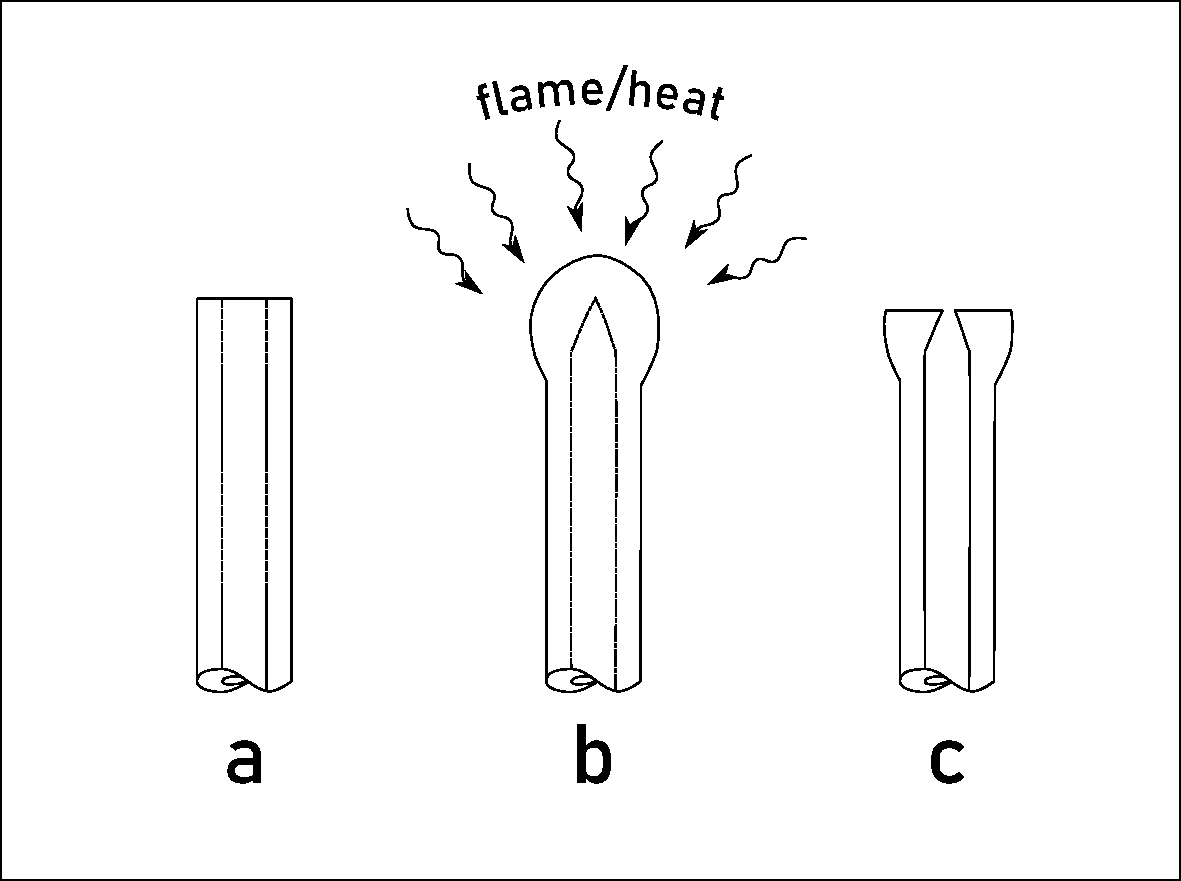
\includegraphics[width=0.5\textwidth]{Figures/Restrictor.pdf}
\decoRule

\caption[A diagram of a integral restrictor.]{The steps of making a Guthrie restrictor. (a) Cut
length of quartz capillary (b) Heat with flame to soften glass and create
internal cone (c) Grind down end to expose orifice of the appropriate size.}

\label{fig:restrictor}
\end{figure}

We found this restrictor robust and fairly simple to manufacture. It was
possible to adjust the flow to a given flow rate. This design of restrictor
should eliminate discrimination, because the decompression takes place in a very
short space, and mostly outside of the capillary.

However, the Guthrie design proved prone to blockage. These blockages could not
be eliminated by incorporating a 0.5 \si{\micro\metre} filter before the restrictor, which
prompted an investigation into the cause of blockages.

To rule out the possibility that it was particles that caused the Guthrie
restrictor to become blocked, we first had to determine the diameter of the
orifice. This proved to be harder than expected: optical microscopy was not able
to give a simple, unambiguous measure of the orifice diameter.

Scanning electron microscopy (SEM) showed that the orifice diameter of a Guthrie
restrictor is about 10 \si{\micro\meter}, as shown in Figure
\ref{fig:restrictororifice} This makes it very unlikely that particles with an
origin in the SFC system blocked the restrictor: even particles from the column
packing material should not block this restrictor.

\begin{figure}
\centering
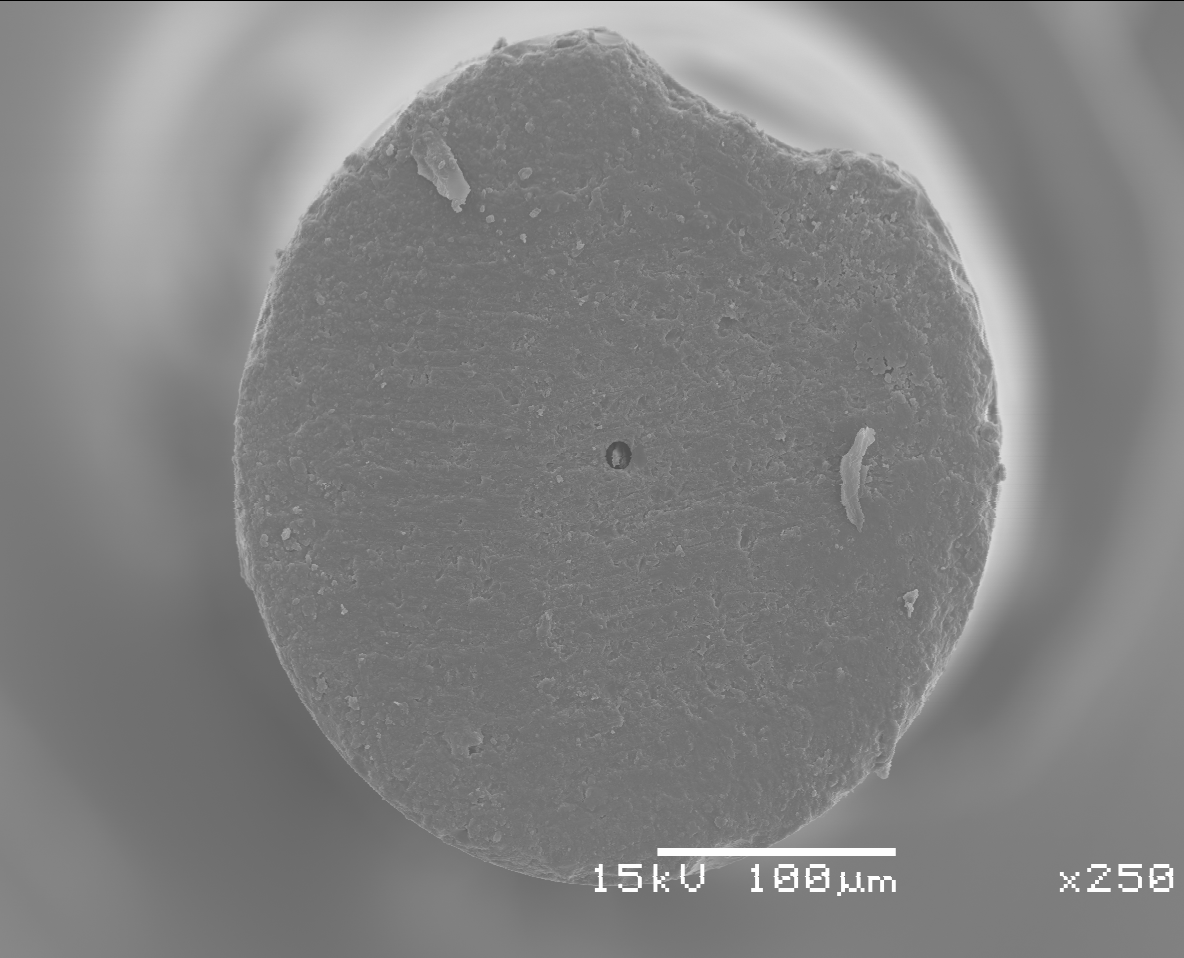
\includegraphics[width=\textwidth]{Figures/sem_h_001.png}
\decoRule

\caption[A electron microscope photo of a restrictor orifice]{An electron
microscope photograph of a restrictor tip, showing the size of the orifice.}

\label{fig:restrictororifice}
\end{figure}

Experience had taught us that the restrictor did not block if the flow was
continuous. It was only when the pressure in the restrictor cycled that
blockages occurred. To eliminate the possibility that it was material from the
stop valve that caused the blockages, we cycled the pressure by switching the
pump on and off, allowing the pressure to bleed off through the restrictor. This
still caused the blockages.

Examination of blocked restrictors with electron microscopy revealed that the
restrictors became blocked by a soft material. Backscatter SEM mode allows the
energy of the backscattered electrons to be measured, which yields information
about elemental composition. While much care must be taken before this
information can be used for quantitation, it is certain that the deposited
material contains significant quantities of carbon and oxygen, and possibly some
chlorine. This points to the probability that the material blocking the column
is organic in nature, and possibly polymeric. See Figure \ref{fig:restrictorblockage}.

\begin{figure}
\centering
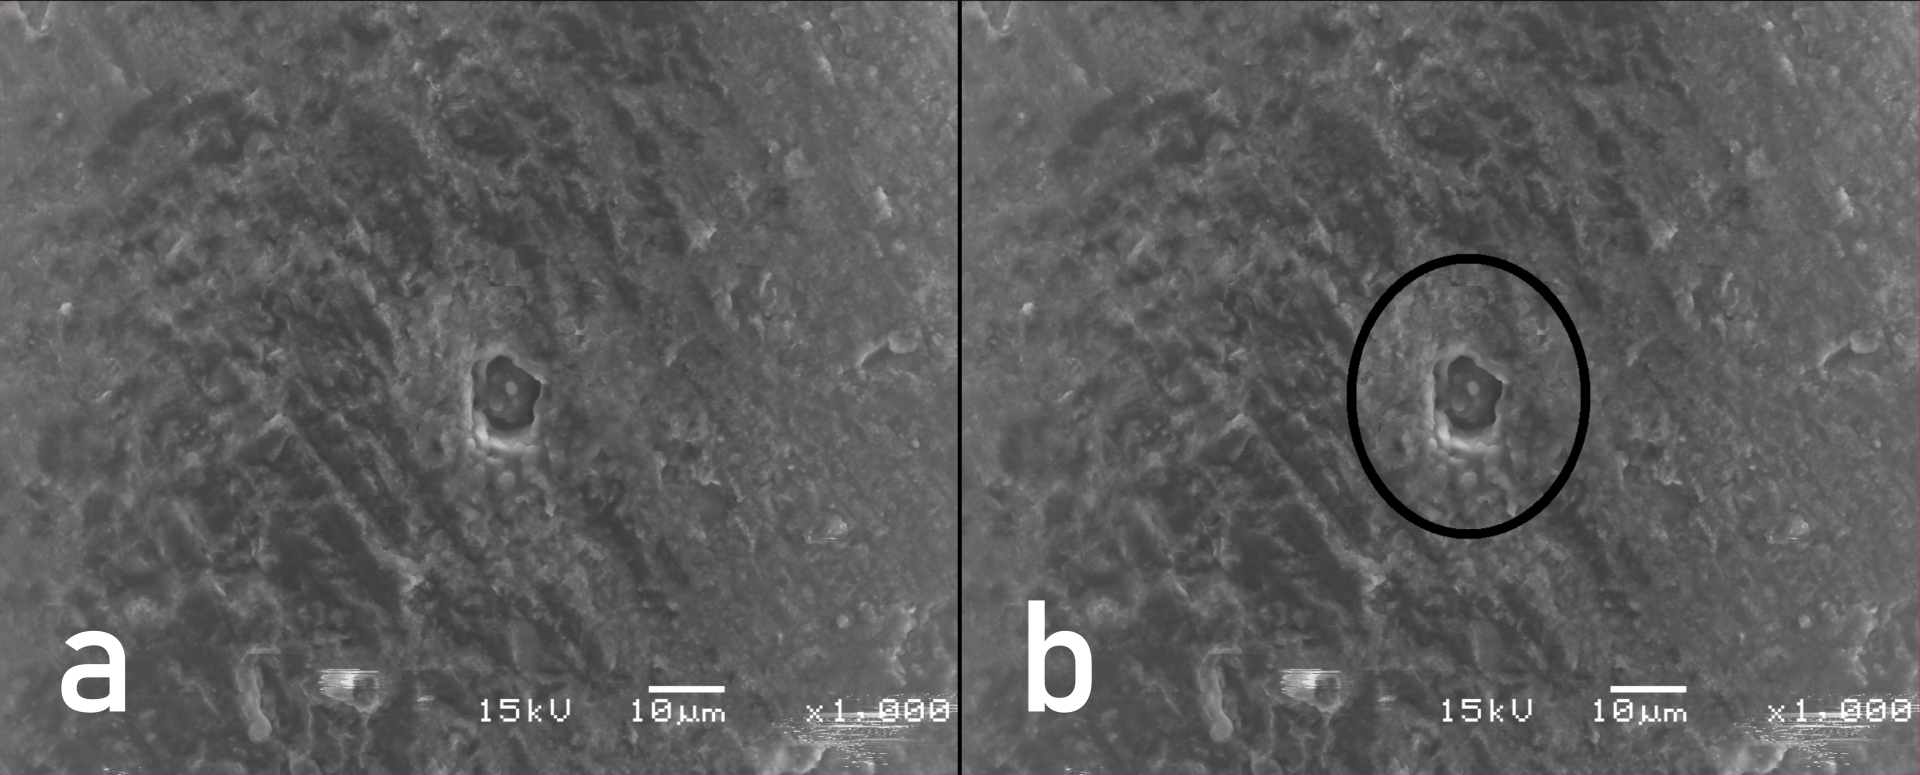
\includegraphics[width=\textwidth]{Figures/Blockage_1920.png}
\decoRule

\caption[A electron microscope photo of a blocked restrictor orifice]{An
electron microscope photograph of a blocked restrictor orifice. (a) Original
image (b) Image with black circle showing estimated original orifice location}

\label{fig:restrictorblockage}
\end{figure}



We could not determine the origin of the material, but it seems likely that it
comes from the column, because without a column there was no blockage. We
eliminated the possibility of blockage by sample material by using a brand new
column. We suspect that it might be remnants of surfactants used in the
synthesis of the silica gel stationary phase that are leached out of the column
packing, and then precipitates in the restrictor when the pressure drops and the
compounds desolvates.

The smallness of the orifice contributes to the plugging problem. With a
diameter of 50 \si{\micro\metre}, a solid sphere that fits in this capillary
will have a volume of .065 \si{\nano\litre}, or 65 \si{\pico\litre}. This means
that nanogram quantities of material can easily block the restrictor.

Being satisfied that an unfortunate combination of restrictor design and column
packing was the likely the cause of the blockages, we decided to choose a
different restrictor design. The choice was a simple linear restrictor and
we trusted that heating the end of the restrictor would prevent discrimination.

The linear restrictor was 800 \si{\milli\metre} long and had an internal
diameter of 0.050 \si{\milli\metre}.

\subsection{Detector}

In this supercritical fluid chromatograph there is no dedicated detector: the
role of the detector is taken by a gas chromatograph. This gas chromatograph
collected fractions from the SFC, and separated them in fast chromatographic
runs with an FID detector, yielding comprehensive 2D chromatograms.

\todos